\documentclass[conference]{IEEEtran}
\IEEEoverridecommandlockouts
% The preceding line is only needed to identify funding in the first footnote. If that is unneeded, please comment it out.
\usepackage{cite}
\usepackage{amsmath,amssymb,amsfonts}
\usepackage{algorithmic}
\usepackage{graphicx}
\usepackage{textcomp}
\usepackage{xcolor}
\def\BibTeX{{\rm B\kern-.05em{\sc i\kern-.025em b}\kern-.08em
    T\kern-.1667em\lower.7ex\hbox{E}\kern-.125emX}}
\begin{document}

\title{Analysis of Pressure Separator Processes and Pressure Relief Valve Devices in Gas Production}

\author{\IEEEauthorblockN{Mai Thanh Hai\textsuperscript{1}, Dinh Hoang Son\textsuperscript{2}, Nguyen Bao Son\textsuperscript{3}}
    \IEEEauthorblockA{\textit{School of Electrical \& Electronic Engineering, Hanoi University of Science and Technology} \\
        Email: \textsuperscript{1}hai.mt210308@sis.hust.edu.vn, \textsuperscript{2}son.dh212417@sis.hust.edu.vn, \textsuperscript{3}son.nb212418@sis.hust.edu.vn}
}


\maketitle

\begin{abstract}
    Gas production is a critical industrial process that requires careful management to ensure both safety and efficiency. This paper focuses on the pressure separator process within gas production systems, highlighting its importance in separating high and low pressure gas. Utilizing an existing Piping and Instrumentation Diagram (P\&ID) as a practical example, the paper delves into the operational intricacies of the pressure separator and the role of pressure relief valve devices in maintaining system safety. The study aims to provide a detailed understanding of the processes and equipment involved, emphasizing the significance of proper pressure management in gas production.
\end{abstract}

\begin{IEEEkeywords}
    gas production, pressure separator process, pressure relief valve, pressure safety valve
\end{IEEEkeywords}

\section{Introduction}

The gas production industry is a cornerstone of the global energy supply chain, necessitating stringent operational protocols to ensure both safety and efficiency. Among the critical components of this industry is the pressure separator process, which plays a pivotal role in distinguishing between high and low pressure gas streams. This paper presents an in-depth analysis of the pressure separator process, utilizing a practical example from an existing Piping and Instrumentation Diagram (P\&ID). Additionally, the study explores the functionality and significance of pressure relief valve devices, which are essential for maintaining system integrity and preventing hazardous overpressure scenarios. By examining these elements, the paper aims to enhance the understanding of pressure management practices within gas production systems, thereby contributing to improved operational safety and efficiency.


\section{Overview of Gas Production}

The production facility examined in this paper is operated by The General Oil \& Gas Operating Company, situated in Chemical City, Texas. This facility handles hydrocarbon fluids extracted from natural gas wells located on production platforms. These wells channel the production fluids into a main production header, which then delivers the feedstock to the facility. During the initial stage of the separation process (high pressure stage), the production fluids are directed into a high pressure separator where the liquid and gas components are separated under specific temperature and pressure conditions. The gas exiting the high pressure separator mainly consists of lighter hydrocarbons and requires no further treatment. This gas is transported via the export gas pipeline to nearby gas processing companies. In the subsequent stage of the separation process (low pressure stage), the liquid from the first stage is transferred to the low pressure separator, where it undergoes flashing at a designated temperature and pressure. The gas stream from the low pressure separator is compressed and then merged with the gas exiting the high pressure separator. The liquid from the low pressure separator is considered stabilized for processing and is pumped into the high pressure export liquid pipeline.

The key equipment utilized in this process, includes a High Pressure Separator, Low Pressure Separator, Export Pump, and Gas Compressor. The Process Flow Diagram (PFD) of the entire gas production facility is shown in Fig.~\ref{fig:PFD}



\section{Four main processes in gas production}
Each of the four main processes revolves around a specific equipment within the studied gas production facility. Those equipment consist of the High Pressure Separator, Low Pressure Separator, Export Pump, and Gas Compressor. The following sections provide a detailed explanation of each process.

\subsection{High Pressure Separator}\label{HPS}
Hydrocarbon fluids enter the high pressure separator (V-101) via a pressure reducing valve (PRV-101A), which lowers the pressure from approximately 700 psig (production header pressure) to 350 psig (first stage operating pressure). The pressure within the separator is regulated by the pressure control valve PV-101B. Flashing occurs inside the vessel, leading to the separation of gas and liquid components. The reduction in flow velocity allows liquid droplets to settle out of the gas stream. The separator vessel provides the necessary retention time for effective gas-liquid separation and also accommodates intermittent liquid surges. The liquid level in the vessel is controlled by the level control valve LV-101A. As the hydrocarbon fluids contact the inlet diverter, most of the liquid falls into the liquid section while the gas flows over the inlet diverter. The gas stream continues to flow horizontally above the liquid section, and small liquid droplets not separated by the inlet diverter are removed by gravity. Liquid droplets too small to be separated by gravity are captured by a de-mister pad. The gas exits the high pressure separator and enters the export gas pipeline to nearby gas processing facilities. Overpressure protection for the high pressure separator is provided by relief valve PSV-101. The P\&ID of the High Pressure Separator is shown in Fig.~\ref{fig:HPS}.


\subsection{Low Pressure Separator}\label{LPS}

% Place figures and tables at the top and bottom of columns. Avoid placing them in the middle of columns. Large figures and tables may span across both columns.

The liquid from the high pressure separator flows into the low pressure separator via the level control valve LV-101A. The low pressure separator operates at 50 psig, allowing lighter hydrocarbons to vaporize and partially stabilize the liquid. The vapor and liquid separate in a manner similar to V-101. The gas is directed to compressor C-104, while the partially stabilized liquid is pumped out by pump P-103. Overpressure protection for the low pressure separator is provided by relief valve PSV-102.


\subsection{Export Pump}\label{EP}

\subsection{Gas Compressor}\label{GC}

\section{Pressure Relief Valve Hardware Device}

\subsection{Structure}

\subsection{Operating Principle}

\subsection{Classification}

\subsection{Application}

\subsection{Advantages and Disadvantages}

\section{Process Flow Diagram}
The process flow diagram (PFD) of the studied system is shown in Fig.~\ref{fig:PFD}.

\begin{figure*}[htbp]
    \centering
    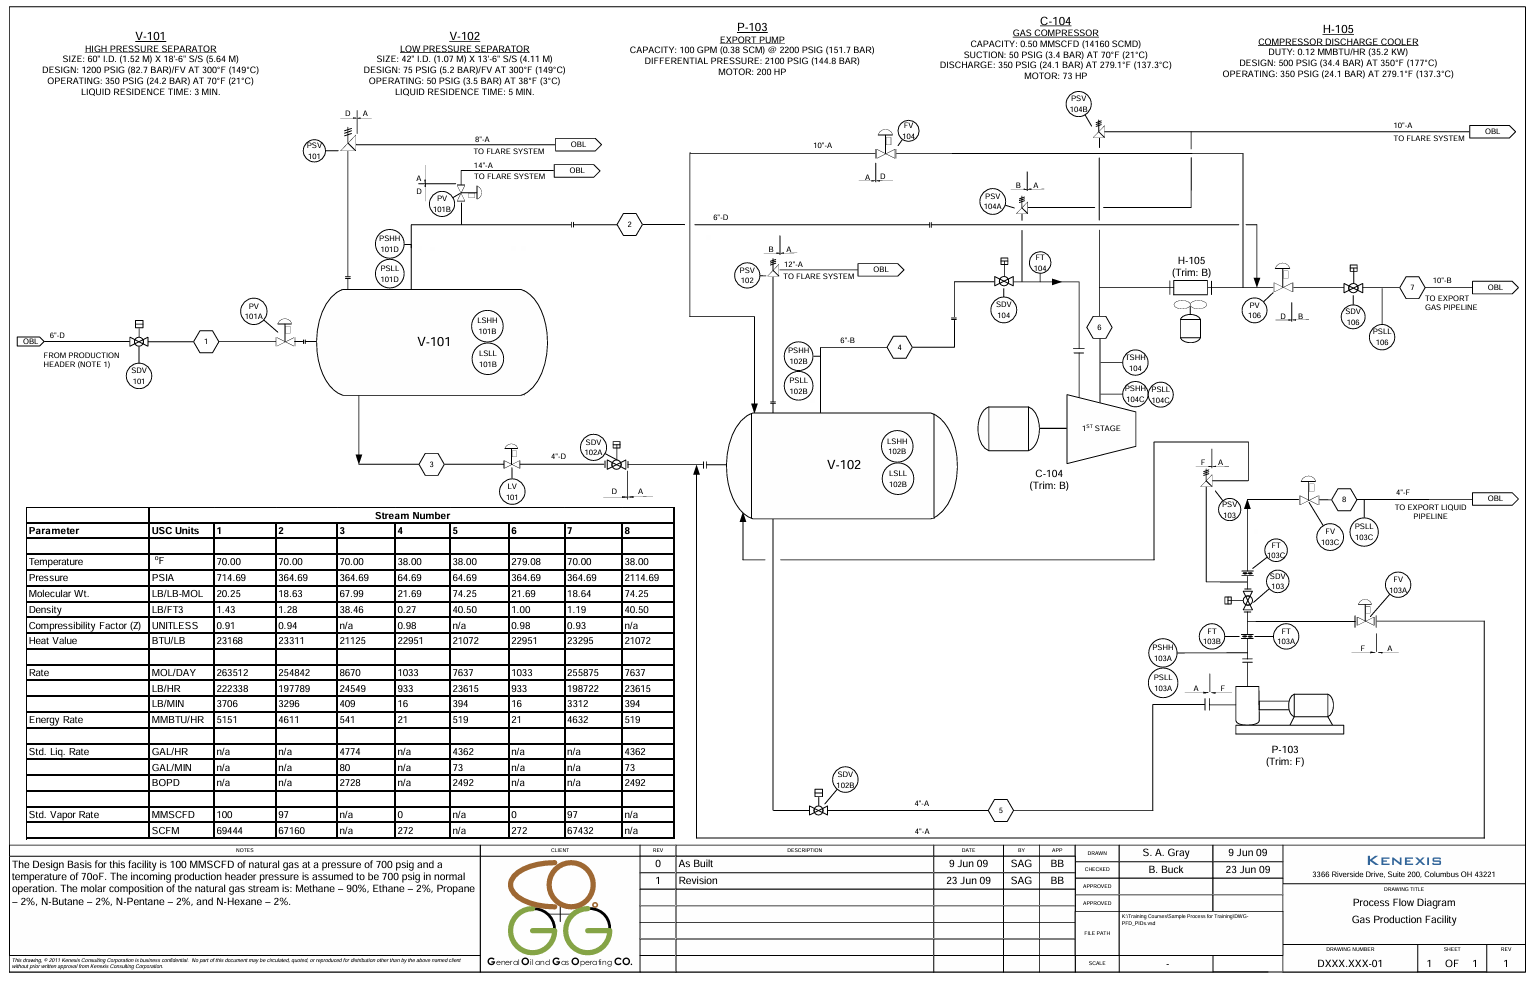
\includegraphics[width=\textwidth]{process_flow_diagram.png}
    \caption{Process Flow Diagram}
    \label{fig:PFD}
\end{figure*}

\section{Piping and Instrumentation Diagram}
The Piping and Instrumentation Diagrams (P\&ID) begin on this page. Fig.~\ref{fig:HPS}--Fig.~\ref{fig:LPS} correspond to the content of sections \ref{HPS}--\ref{GC}.

\begin{figure*}
    \centering
    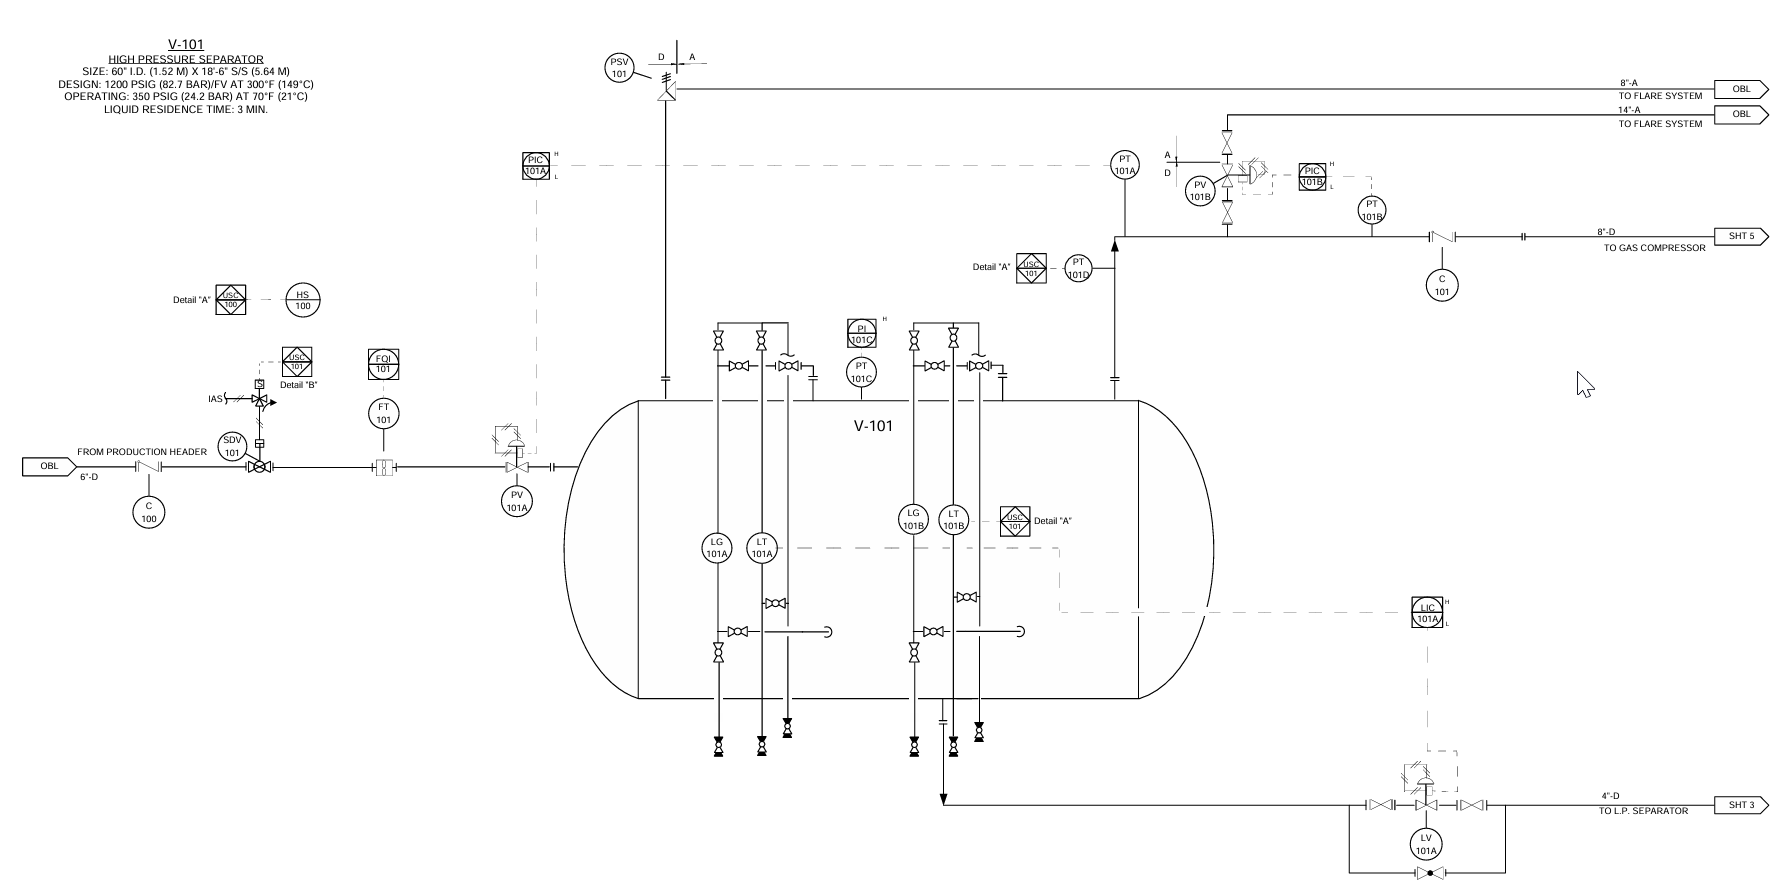
\includegraphics[width=\textwidth]{high_pressure_separator.png}
    \caption{High Pressure Separator}
    \label{fig:HPS}
\end{figure*}

\begin{figure*}[htbp]
    \centering
    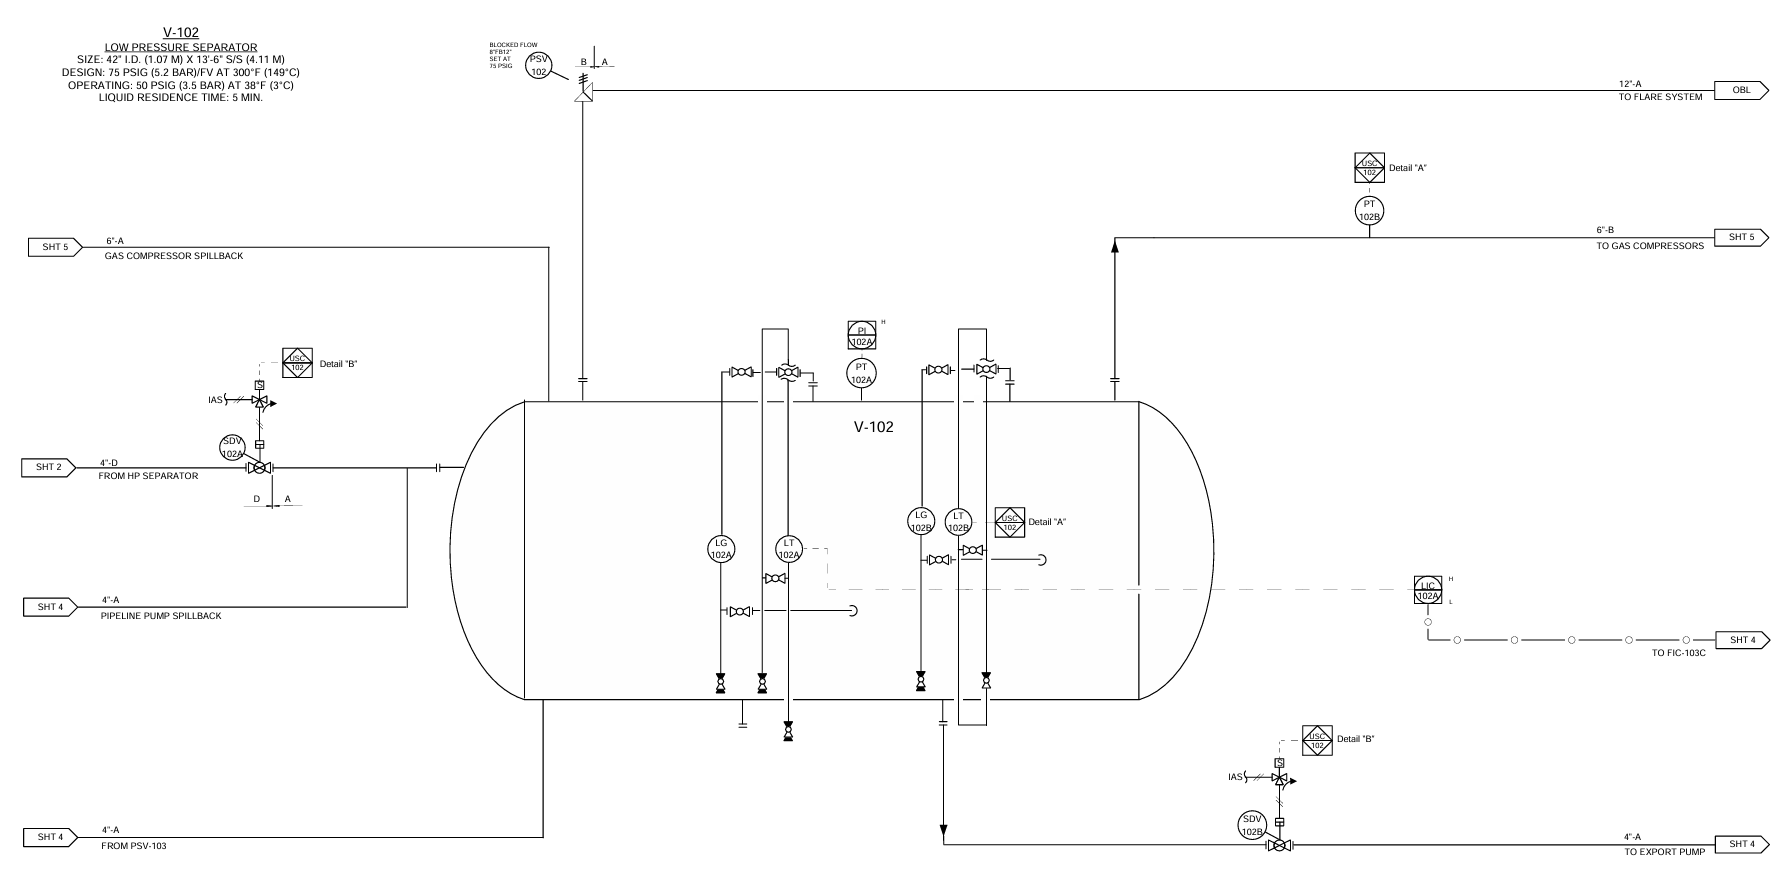
\includegraphics[width=\textwidth]{low_pressure_separator.png}
    \caption{Low Pressure Separator}
    \label{fig:LPS}
\end{figure*}


\section*{Acknowledgment}

The authors would like to sincerely thank Mrs. Dinh Thi Lan Anh for her guidance and support throughout the EE35550E course ``Process Control''during the 2024.1 semester at Hanoi University of Science and Technology.

\begin{thebibliography}{00}
    \bibitem{Kenexis} SA Gray and B Buckeye, ``Training Course Packet for Gas Production Facility ,'' Kenexis Consulting, June 2011.

\end{thebibliography}

\end{document}
